\section{Methodology}
In this section, we explain our setup for determining Mamba's ability to learn
from context.
In our experiments, we test 2 different models which attempt to use Mamba for its
in-context learning abilities against a variety of datasets, elaborated on
below.

\subsection{Data}
In this paper, we train our models to predict text labels in a type of task that
we will call \textbf{in-context OCR}.
A single instance of an in-context OCR task consists of a set of images of text,
and the task is to assign labels to these images.
The difference between in-context OCR and standard OCR is that with in-context
OCR, each instance consists of multiple images in the same context.
This means that in theory, an agent predicting this task can benefit by
using context clues from different parts of the image.

With our models, we train them to solve this task in an autoregressive manner.
That is, the prediction for each character in each label is based on the
previous characters and previous image/label pairs.

In all of our datasets, we rescale each image to a height of 32 pixels.

\subsubsection{Position Encoding}
An issue with in-context OCR as outlined above is that the model is not
provided any information about the scale and relative position of each word.
As such, we append rotational positional encodings similar to the ones used in
the transformer architecture\cite{attention} in each word such that each
pixel embeds its relative position within the original image.
With these positional encodings, a model can now directly access the position of
any given image, and it can infer the scale of each image by evaluating the
change in position between the corners of the image.

\subsubsection{Text Injection}
\begin{figure}[ht]
    \begin{center}
    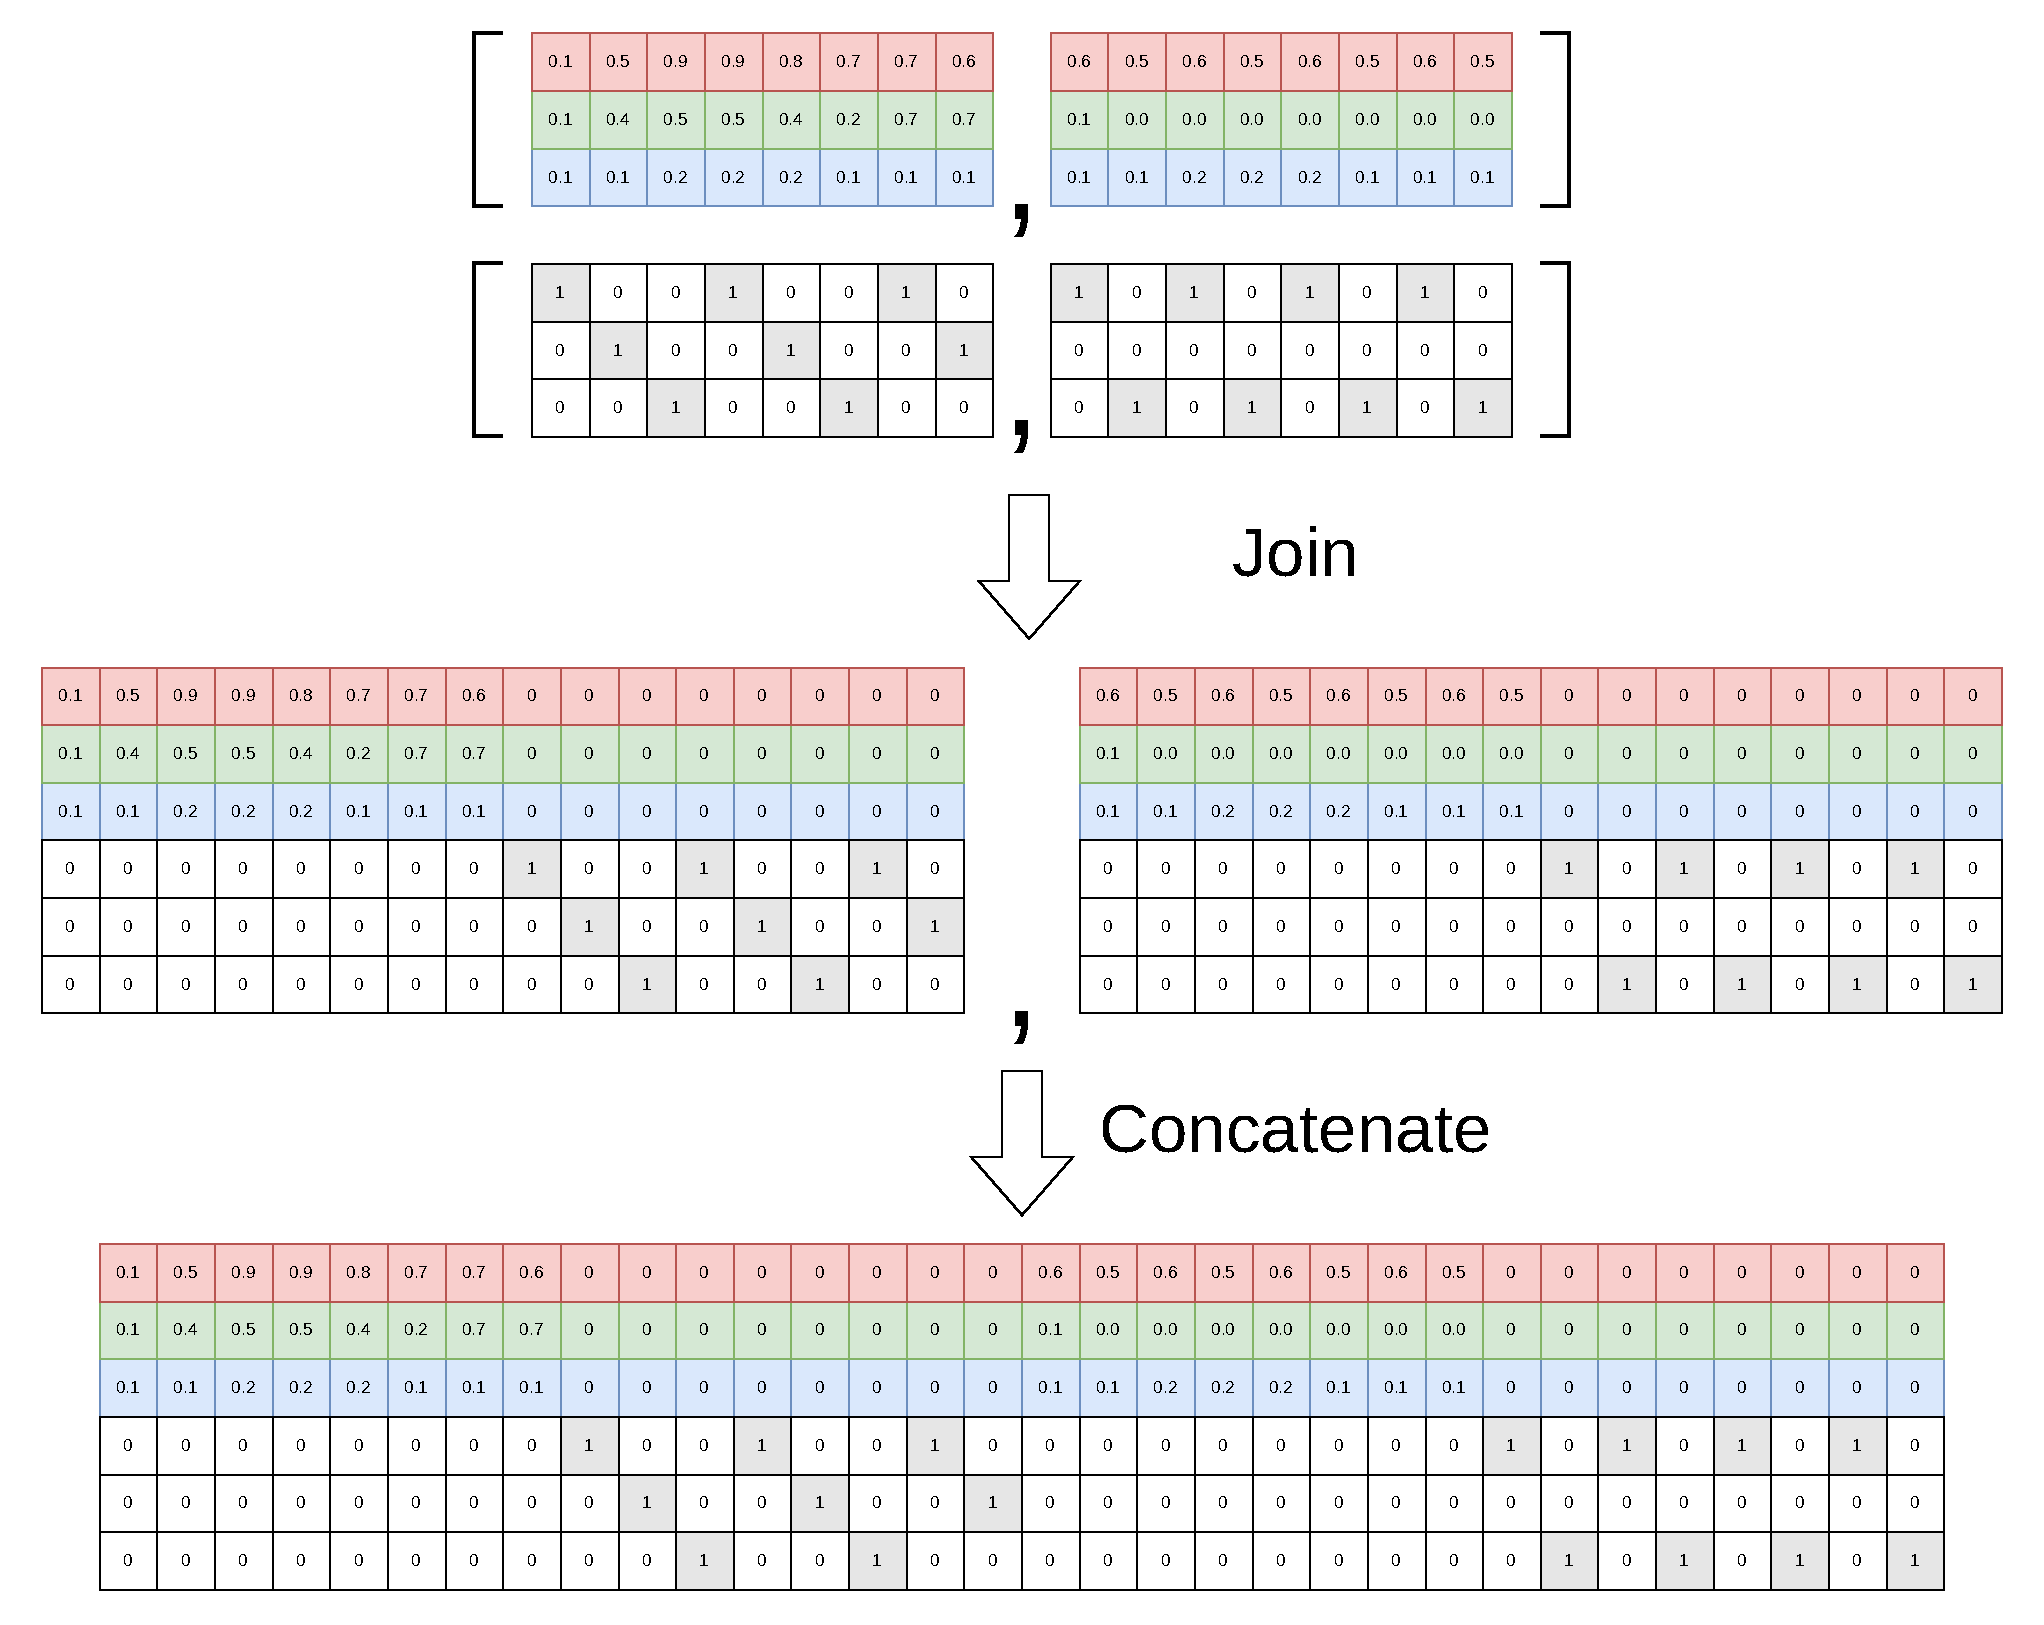
\includegraphics[width=0.5\textwidth]{figures/in_context_encoding.pdf}
    \end{center}
    \caption{In-Context Encoding}
    \label{incontextencoding}
\end{figure}

In order to supply context to the models, we encode our dataset using a scheme
that involves what we will call in-context encoding.
Before in-context encoding, all of the images within a context need to be
transformed into sequences.
We will call these sequences the image matrices, where each column corresponds
to a pixel in the image(with positional encodings and other per-pixel metadata)
Then, we encode the labels as one-hot tokens such that each label is represented
as a matrix of one-hot columns.
We now apply the in-context encoding transformation on these 2 lists of tensors.
First, we diagonally append the label tensors to the image sequence tensors such
that they are in separate channel spaces.
Then, we append all of the combined tensors lengthwise to get the final tensor.
This process is shown in Figure \ref{incontextencoding}.

With this encoding scheme, we assume that the data is being processed by an
auto-regressive model, where each output token is evaluated based on the
previous (correct) output tokens, and previous predictions in context.

We hypothesize that Mamba's ability to do in-context learning\cite{mamba} will
allow model architectures containing Mamba to perform well on in-context
image prediction.

\subsubsection{MSCOCO-Text}
The first dataset that we use is the COCO-Text dataset, based on the MS COCO
dataset\cite{cocotext}\cite{mscoco}.
This dataset consists of a set of 63k images with each instance of text labeled
with the text string, an axis-aligned bounding box, and a bounding polygon.

The processing that we perform in order to convert this into an in-context OCR
task is fairly straightforward.
First, we filter the dataset to only contain "normal" examples. In particular,
we remove instances that have any of the following problems:
\begin{itemize}
    \item Instance resolution is too low(AABB height less than 32).
    \item Aspect ratio is bad(width is not between 0.5 and 1.5 times the height
    times the number of characters).
    \item Label is a single character or contains more than 10 characters(since
    single characters are usually hard-to-discern punctuation and more than 10
    characters could stretch the models' ability to memorize).
\end{itemize}
Next, we remove any contexts that contain 1 or 0 words. This is since these
instances don't effectively test in-context learning.
Unfortunately, this still misses a few bad samples and shrinks the dataset down
to 439 contexts, which greatly increases the risks of overfitting.
After filtering, for each text instance, we crop the image to the AABB corresponding to
the instance.
If the bounding polygon happens to be a quadrilateral, we instead project the
bounding polygon onto a rectangle with the same dimensions as the AABB.
Then, we proportionally scale the cropped image so that the height is 32.
Finally, for each pixel, we calculate the coordinates that we want to encode
using to the following formulas:
\begin{align*}
    x_{\text{relative}} &= x & x_{\text{absolute}} &= \frac{x_{BB} + x \cdot w_{BB}}{w}\\
    y_{\text{relative}} &= y & y_{\text{absolute}} &= \frac{y_{BB} + y \cdot h_{BB}}{h}\\
\end{align*}
, where $x$ and $y$ are the normalized coordinates of the pixel within the cropped
images($x \in [0, 1]$, $y \in [0, 1]$), $w, h$ are the width and height of the
image in pixels, and $x_{BB}, y_{BB}, w_{BB}, h_{BB}$ are the left edge, top
edge, width, and height of the AABB in pixels.

We append these positional encodings as new channels alongside the red, green,
and blue channels.

For the labels, we encode each character as a one-hot token and add a special
ending character so that the model learns to terminate words.

\subsubsection{Synthetic Words}
\begin{figure}
    \begin{subfigure}{0.5\textwidth}
        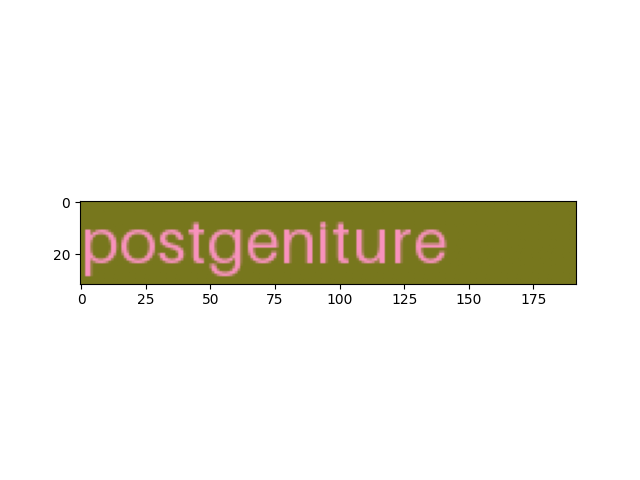
\includegraphics[width=\textwidth]{figures/synthetic_words_example.png}
        \caption{An example image from the synthetic words dataset}
        \label{syntheticwordsexample}
    \end{subfigure}\begin{subfigure}{0.5\textwidth}
        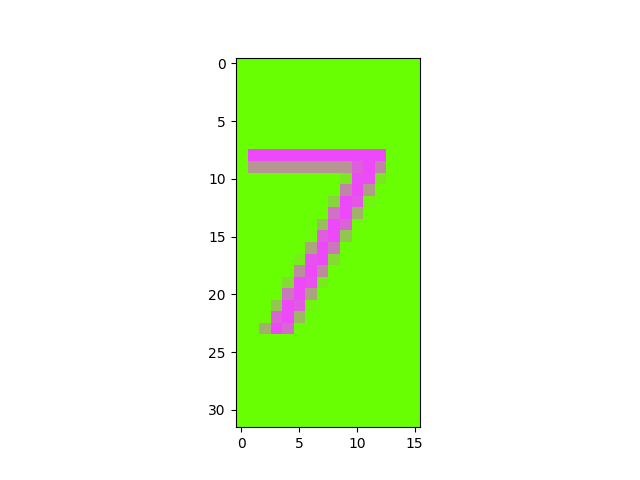
\includegraphics[width=\textwidth]{figures/synthetic_digits_example.png}
        \caption{An example image from the synthetic digits dataset}
        \label{syntheticdigitsexample}
    \end{subfigure}
    \caption{Examples from the synthetic datasets}
    \label{syntheticexamples}
\end{figure}
Since the COCO-Text dataset contains very few "good" images, we construct a
synthetic dataset that serves as a toy example for in-context tasks.
In this dataset, each context is generated using 10 words randomly sampled from
the GNU Collaborative International Dictionary of English\cite{gcide} along with
a random foreground and background color.
Each image consists of the text printed on a solid background, with the
aforementioned colors.
Images within the same context have the same foreground and background color,
but images in different contexts might have different colors.
Like with COCO-Text, the label strings in this datasets are ended with a special
terminator character.
An example is shown in Figure \ref{syntheticexamples}\ref{sub@syntheticwordsexample}.
It is also important to note that positional encodings are omitted since there
is no "original" image that the text instances are placed in.

In-context learning for this dataset would mean memorizing what
foreground/background mean within a dataset.

\subsubsection{Synthetic Digits}
This dataset is similar to the synthetic words dataset, except that instead of
entire words, this dataset is just images of single letters.
In addition, the labels are not terminated, since they are all the same length.
An example is shown in Figure \ref{syntheticexamples}\ref{sub@syntheticdigitsexample}

\subsection{Models}
In our experiments, we evaluate 2 models.

\subsubsection{Sequence Stack}
\begin{figure}[ht]
    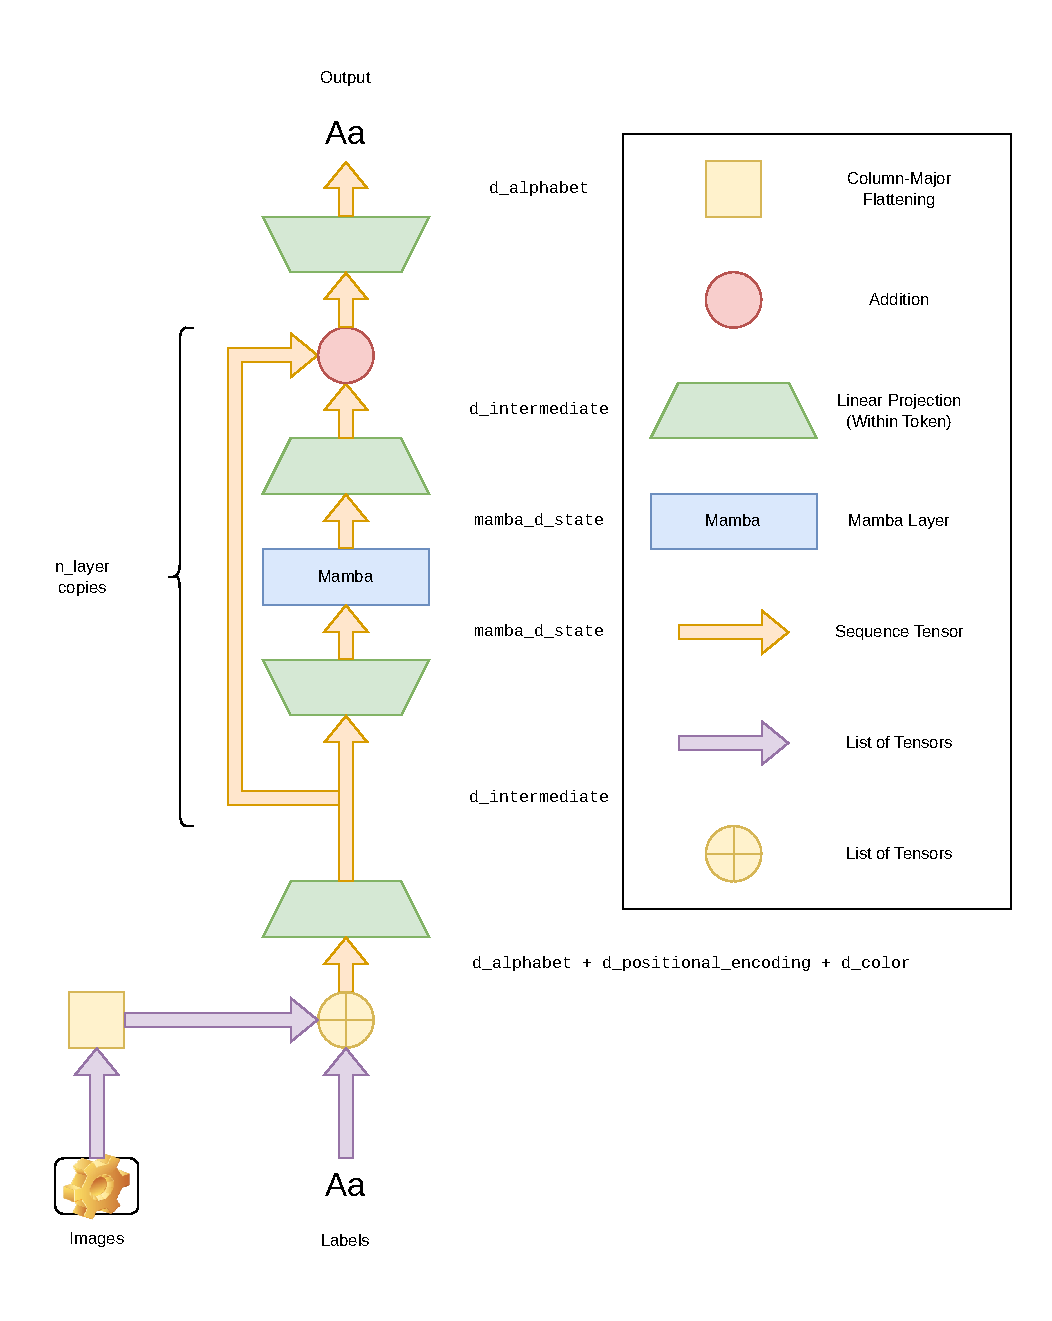
\includegraphics[width=\textwidth]{figures/sequence_stack.pdf}
    \caption{Sequence Stack Architecture}
    \label{sequencestack}
\end{figure}
The first model architecture that we test is a multi-layer Mamba architecture.
The method used for converting images is column-wise flattening. That is, we map
pixels in the image to tokens in the sequence such that each pixel is placed
next to the pixel directly above and below.
These 
The full architecture is shown in Figure \ref{sequencestack}.

\subsubsection{MedMamba}
\begin{figure}[ht]
    \begin{subfigure}{0.5\textwidth}
        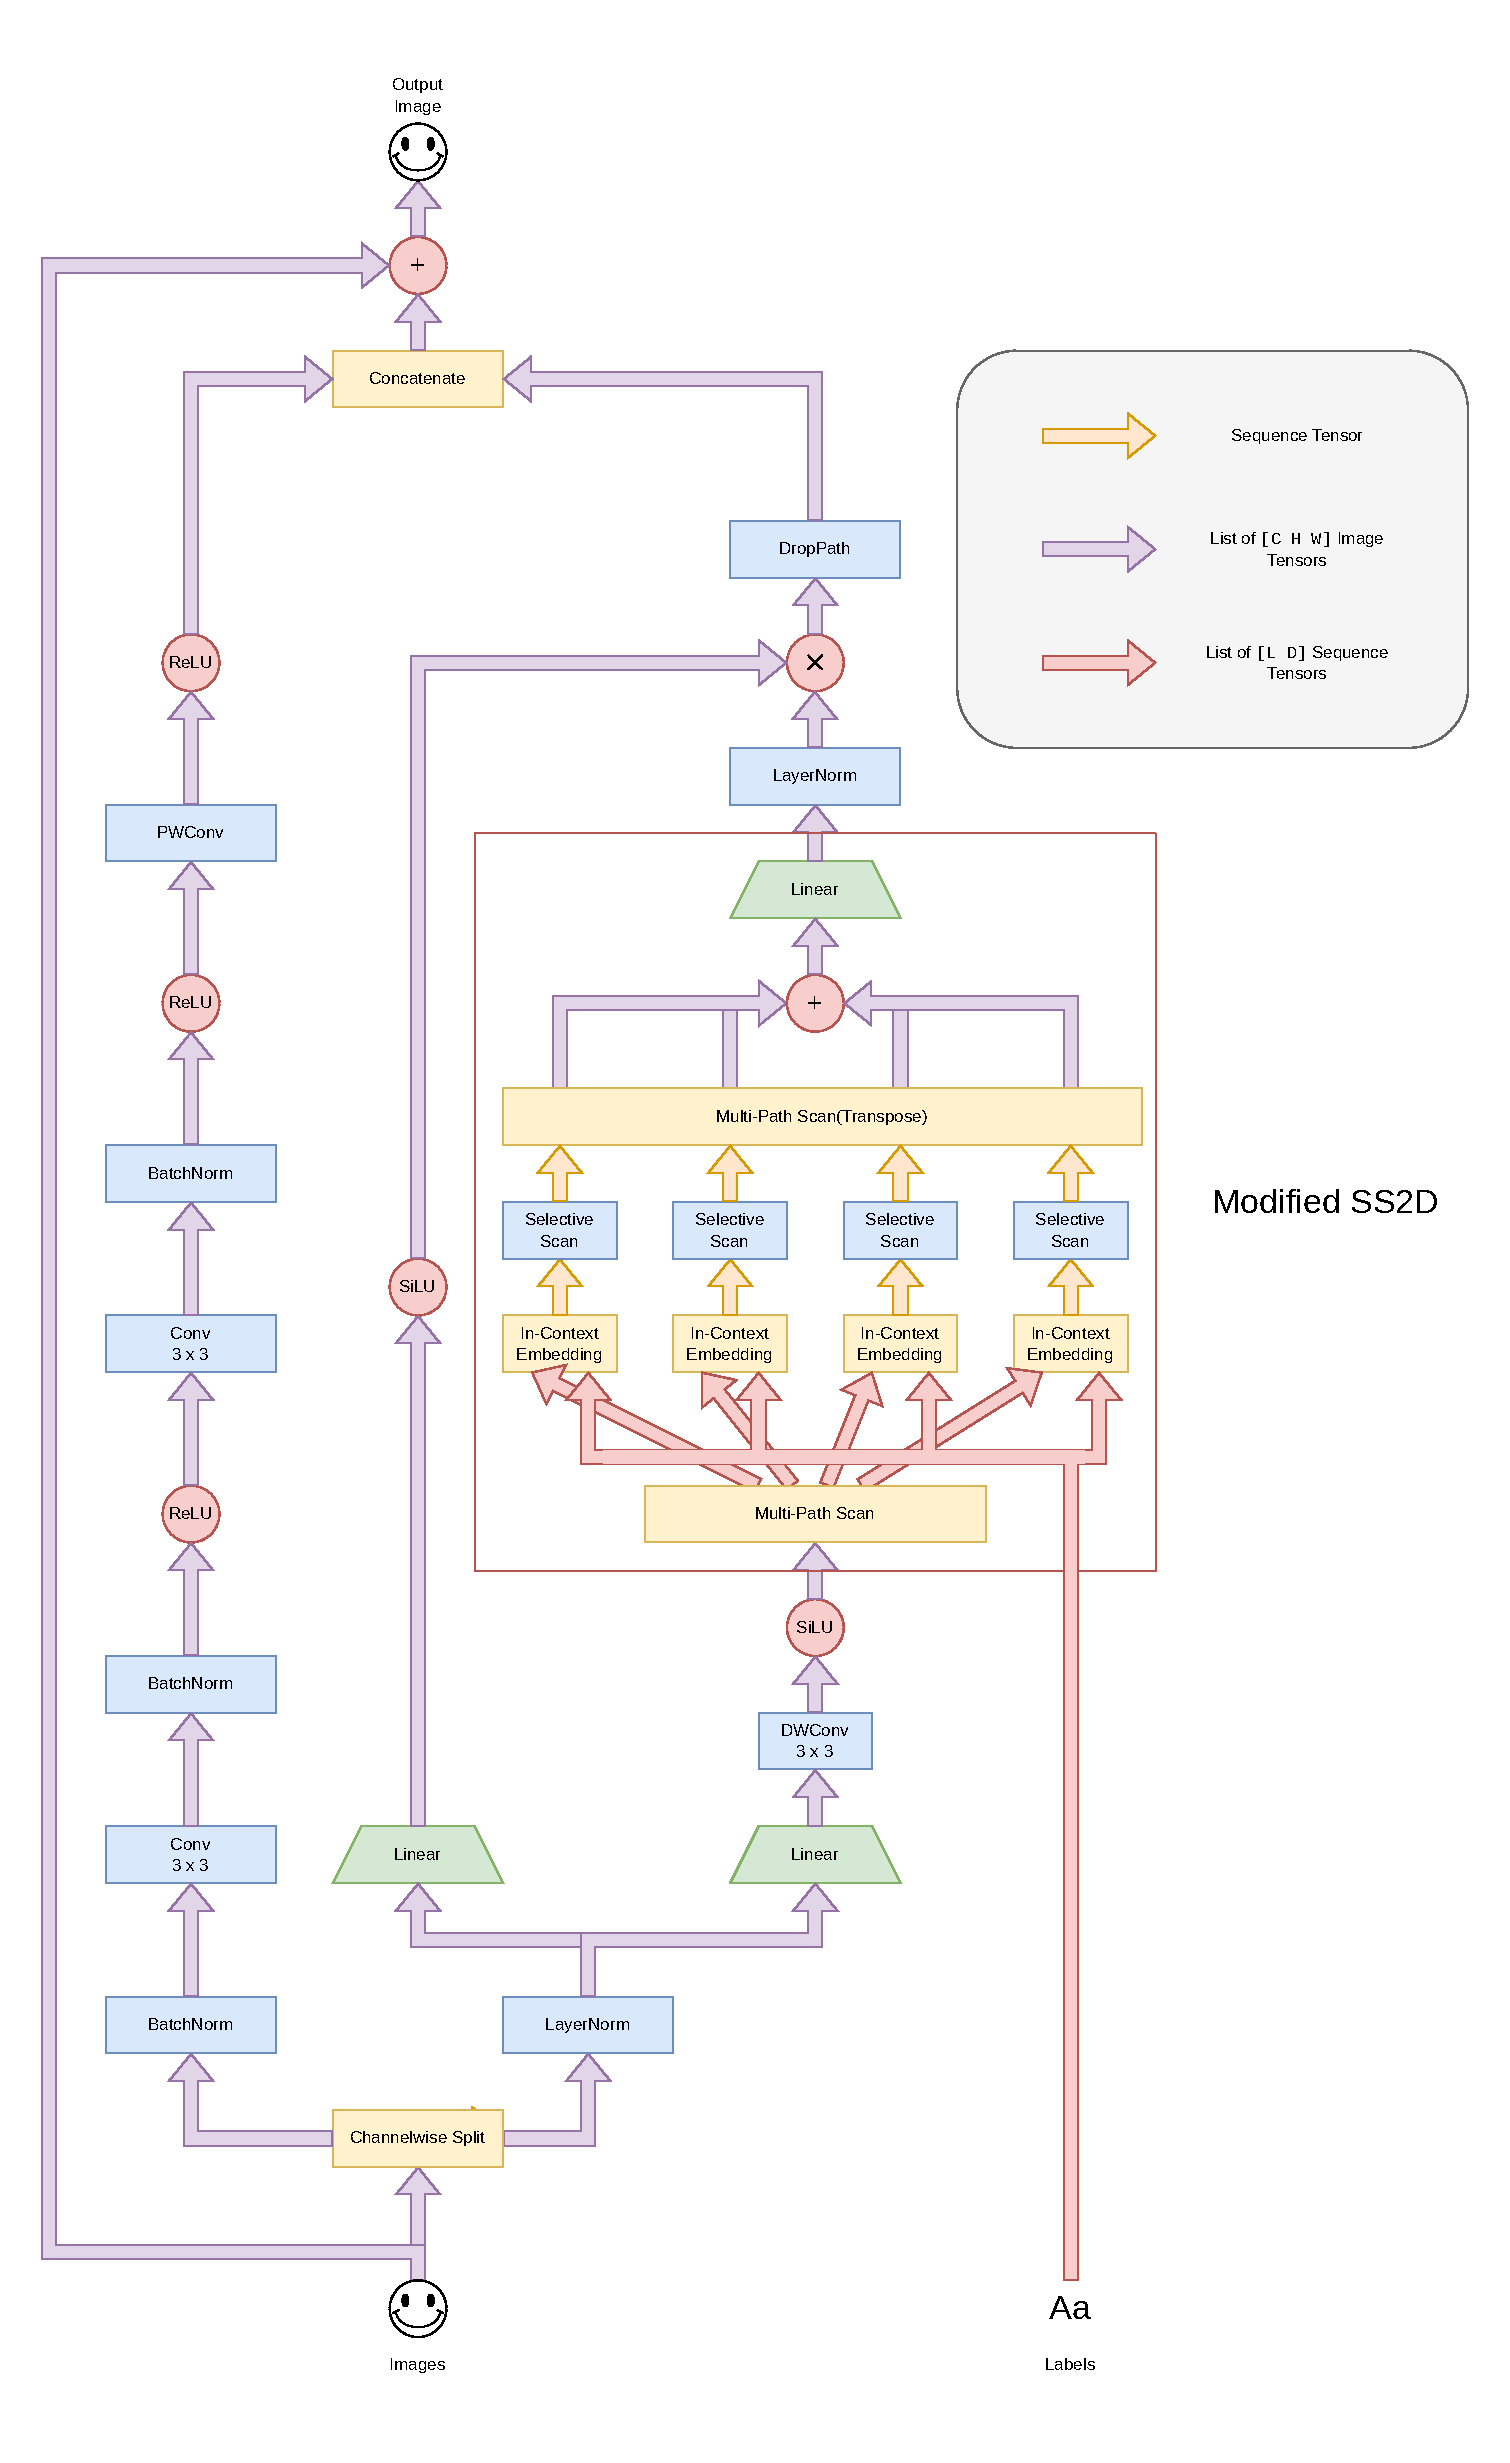
\includegraphics[width=\textwidth]{figures/ss_conv_ssm.pdf}
        \caption{SS-Conv-SSM with Context Injection}
        \label{medmambastacklow}
    \end{subfigure}
    \begin{subfigure}{0.5\textwidth}
        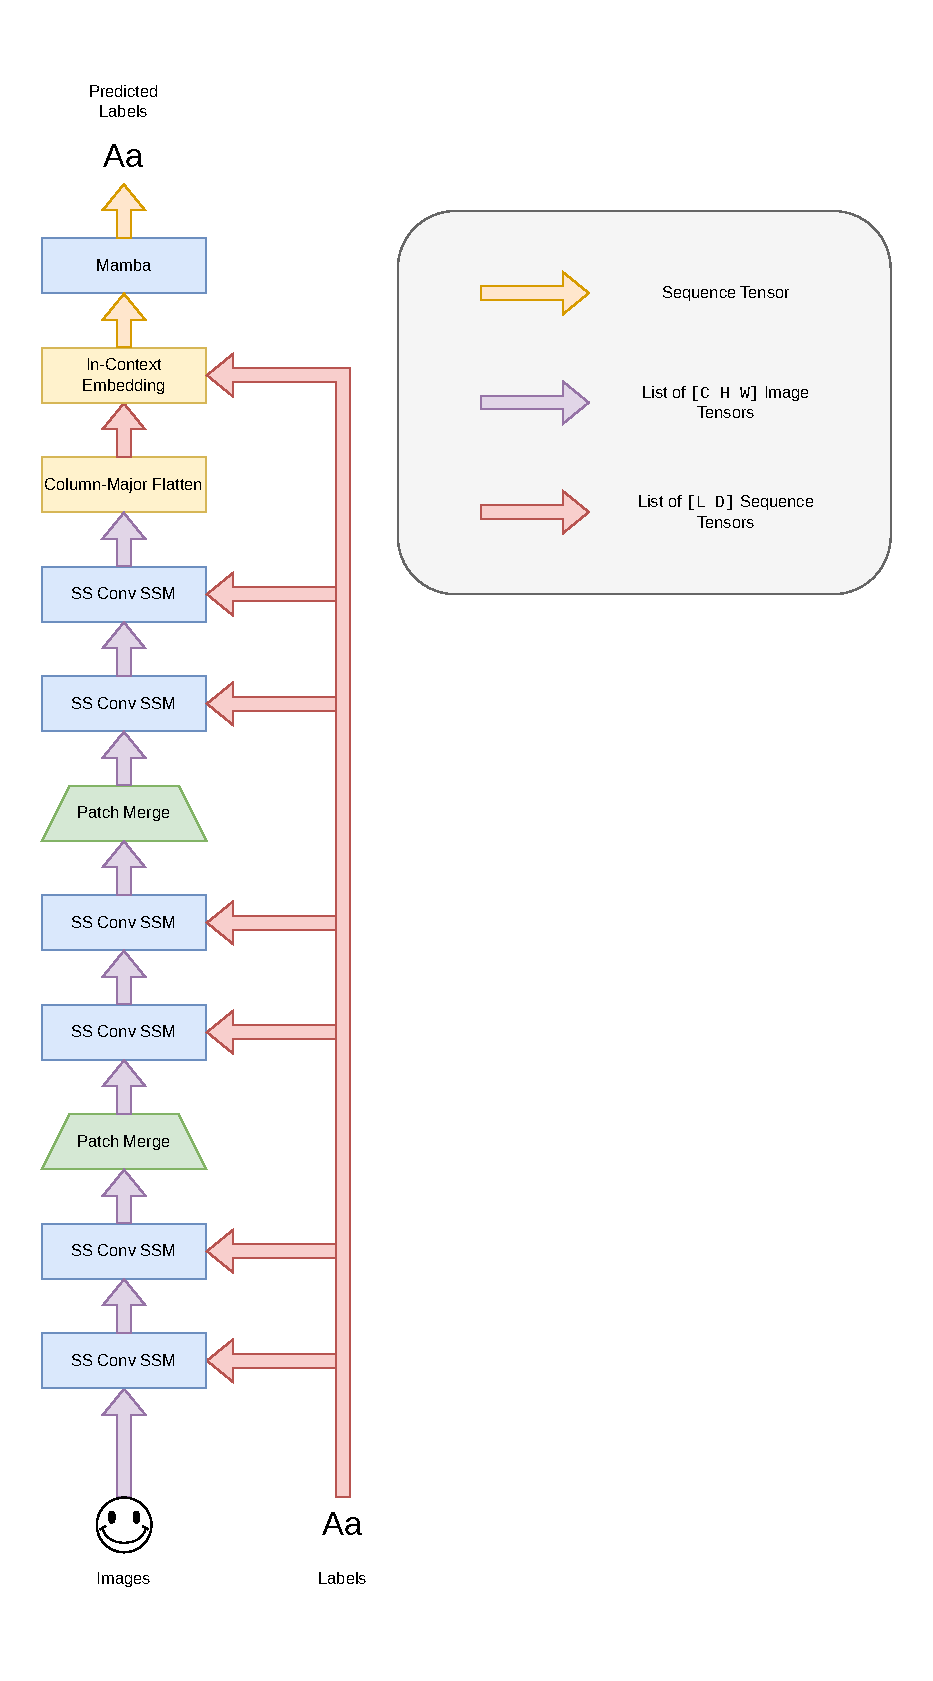
\includegraphics[width=\textwidth]{figures/medmamba_stack.pdf}
        \caption{High-Level MedMamba stack structure}
        \label{medmambastackhigh}
    \end{subfigure}
    \caption{MedMamba}
    \label{medmambastack}
\end{figure}
Another model architecture we look at is based on the MedMamba
architecture\cite{medmamba}.
The main difference between MedMamba's architecture and our architecture is that
We modify the SS2D block(boxed in red in Figure \ref{medmambastacklow}) to include context injection for each scanning
path.
Since context injection adds new channels, we also add a linear layer to the
output of the SS2D block to ensure that the number of channels matches the
number of channels in the gating vector.

Like MedMamba, we use Patch Merging layers(originally introduced by the SWin
Transformer architecture \cite{swintrans}).
